\section{The Wollok Language}
\label{sec:wollokLanguage}

% Free form, variable number of sections, technical details.
% But in general do not mix solution and discussions/possible variation let that for discussion

Wollok is a brand new language, built to specifically give support to our pedagogical approach. 
Wollok provides aextremely simple programming model, which allows the students to create programs that including objects, messages and polymorphism, but without the need for more abstract concepts such as classes, inheritance or type annotations.
Later in the course, Wollok allows for the incremental introduction of more abstract concepts,
providing a smooth transition into a full-fledged OO programming model.

The example in figure \ref{fig:helloWorld/wollok} shows an example first program in a Wollok-based OO introductory course.
Syntax has been reduced to a minimum and the basic constructs of the language match exactly the concepts we want to transmit, \eg \code{var} is used to define variables and \code{method} is used to define methods.
The \code{accumulator} object is defined as a stand-alone (\ie it has no visible class), automatically instantiated and \emph{well-known} (\ie globally accesible) object (WKO).

\begin{figure}[ht]
 \centering
 \begin{lstlisting}[language=Wollok]
	object accumulator {
		var total = 0
		
		method getCurrentTotal() { return total }
		method add(amount) { total += amount }
	}
 \end{lstlisting}
 
 \caption{\small Sample initial Wollok program.}
 \label{fig:helloWorld/wollok}
\end{figure}

\medskip 

We put special emphasis in avoiding input and output (I/O). 
Normally, writing to standard output as it is shown in Fig. \ref{fig:helloWorld} will be considered a problem in industrial software construction.
Therefore, teaching our students to try out their programs in this way is introducing a bad practice that will have to be \emph{unlearned} later.
On the other hand, we need some kind of user interaction to be able to see the behavior of our programs and proper handling of user interaction is way beyond the scope of an initial OO course.

The first tool we introduce to try out a program without requiring I/O is a \emph {read-eval-print-loop} (REPL). Running a program in the REPL brings all defined objects to live and allows the user to interact with them sending messages, as shown in Fig. {fig:repl}. 
The REPL handles all I/O and the student is only required to write the desired \emph{domain object}.

\begin{figure}[ht]
 \centering
 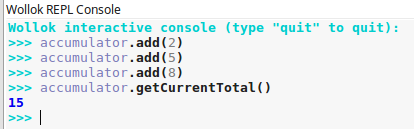
\includegraphics[scale=0.6]{images/accumulator-repl.png}
 \caption{\small Sample usage of the accumulator program in the REPL}
 \label{fig:repl}
\end{figure}


%This is also consistent with some modern industrial OO languages that allow to define both classes or standalone objects, such as Scala \cite{Oder04a}.

%To build this first program students are not required to know about typing, scoping or packaging.
%The only required construct is the \code{program} and the only command is a message send.
%Both the receiver and the parameters are built-in objects which will be handled in the same way as user-defined objects.
%The concepts required to understand this program are no more than program, object, message and argument passing.

Shortly after in the course, we introduce unit testing which slowly replace the REPL as the main form of interacting with objects. Figure \ref{fig:test} shows a sample test for the previous program. 

\begin{figure}[ht]
 \centering
 \begin{lstlisting}[language=Wollok]
 	import accumulator.*

	test "adding 2+5+8 should give 15" {
		accumulator.add(2)
		accumulator.add(5)
		accumulator.add(8)
		assert.equals(15, accumulator.getCurrentTotal())		
	}
   
	test "accumulator starts with 0" {
		assert.equals(0, accumulator.getCurrentTotal())
	}
 \end{lstlisting}
 
 \caption{\small Sample test Wollok program.}
 \label{fig:test}
\end{figure}

Again here Wollok is fine-tuned for our pedagogical objectives.
For example, tests have to be written in a separate file, which introduces the student into some basic knowledge of modularization.
Also, the test runner guarantees that there is no interaction between tests: the messages sent to the accumulator in the first test will not affect the state of the accumulator in the second test\np{sería lindo tener una cita a alguna regla de unit testing que proponga esto}.

\medskip
% Misceláneos
% Profundizar y pulir el highlighting the conceptos primarios y la estratificacion de conceptos
Another simple feature that is very helpful in the initial steps of the course is the presence of literals for lists (\eg \code{[1,2,3]}) and sets (\eg \code{\#\{1,2,3\}}).
This allows us to increase the complexity of examples that we can build without introducing classes.
For example, our \code{accumulator} object can be implemented as shown in Fig. \ref{fig:accumulator/list}.
%Also \emph{Collection literals} reduce boilerplate on object creation, 
%since we think that the excess of bureaucracy to create an object helps to build up 
%the belief that using objects or collections is far more complicated than using numbers or strings, which in turns leads to \emph{primitive obsession} \cite{fowler_refactoring:_1999}.

\begin{figure}[ht]
 \centering
 \begin{lstlisting}[language=Wollok]
	object listBasedAccumulator {
		var history = []
		
		method getCurrentTotal() { 
			return history.sum() 
		}
		method add(amount) { history.add(amount) }
	}
 \end{lstlisting}
 
 \caption{\small Another accumulator implementation, using a list.}
 \label{fig:accumulator/list}
\end{figure}

\medskip
Next in the course, we introduce classes.
Once more, Wollok helps us in the transition: any pre-existent stand-alone object can be converted into a class by just changing the keyword \code{object} for \code{class}\footnote{As a matter of fact, we will also change the name, as our code convention mandates lowercase names for objects and uppercase names for classes}, as shown in Fig. \ref{fig:accumulator/classes}.

\begin{figure}[ht]
 \centering
 \begin{lstlisting}[language=Wollok]
	class ListBasedAccumulator {
		var history = []
		
		method getCurrentTotal() { 
			return history.sum() 
		}
		method add(amount) { history.add(amount) }
	}
 \end{lstlisting}
 
 \caption{\small A third accumulator implementation, class based.}
 \label{fig:accumulator/classes}
\end{figure}

\medskip
Figure \ref{fig:polymorphism} shows how the three previous definitions of accumulator can be used polymorphically. 
Also it shows the usage of more advanced list messages and closures\footnote{In our approach, we introduce polymorphism and closures \emph{before} classes. For reasons of space we skipped those intermediate examples here.}.
A special mention has to be made about the fact of stand-alone objects being used in the same program and even being polymorphic with class-based objects.

\begin{figure}[ht]
 \centering
 \begin{lstlisting}[language=Wollok]
 	import accumulator.*

	test "adding 2+5+8 should give 15" {
		const accumulators = [ 
			accumulator, 
			listBasedAccumulator,
			new ListBasedAccumulator()
		]

		accumulators.forEach { accum =>
			accum.add(2)
			accum.add(5)
			accum.add(8)
			assert.equals(15, accum.getCurrentTotal())	
		}
	}
 \end{lstlisting}
 
 \caption{\small Simple polymorphism example.}
 \label{fig:polymorphism}
\end{figure}


\bigskip 
% Effect
\np{Esto requeriría una mención en la intro, o en general una explicación más detallada.}
Another concept we propose to emphasize in the first programming courses is the control of side effects, 
\ie a programmer should be aware of the potential side effects of each portion of code.
The most basic feature in Wollok to control side effects is the ability to 
differentiate variables (defined using \code{var})
from constants (defined using \code{const}).
One step forward is to incorporate an \emph{effect system} \cite{nielson_type_1999}, \cf Sec. \ref{sec:furtherWork}.
